\documentclass[handout,nooutcomes]{ximera}
%handout
%wordchoicegiven
%space
%nooutcomes
\title{Math 160 Lab 2}
\author{Ben Sencindiver} %Used Bart Snapp and Jim Fowler's mooculus textbook as a guide
\input{preamble.tex}

\outcome{Define linear approximation as an application of the tangent to a curve.}
\outcome{Find the linear approximation to a function at a point and use it to approximate the function value.}
\outcome{Identify when a linear approximation can be used.}
\outcome{Label a graph with the appropriate quantities used in linear approximation.}
\outcome{Find the error of a linear approximation.}

\begin{document}

\section{Math 160 Lab 2 \\ Linear Approximation}

%% Have to edit the date here.
\begin{abstract}
This is Lab 2 for Math 160 - Due Wednesday, March 16, 2017 (NEED TO EDIT). This lab will cover ``linear approximations'': what are they, how do you compute them, and how are they useful. For example, we use linear approximations to estimate the value of (complicated) functions at a given point.\\

Unless stated otherwise, compute all values to $6$ decimal places.
\end{abstract}

\maketitle

\bigskip


%% Start with multiple choice picture question about what SHOULD a linear approximation look like?



Suppose you want to approximate the function $f(x) = (x-2)^2  + 4$ at $x=3$.

Let's explore what properties we would want from this approximation.

It may be helpful to see the point at which you'd like to approximation. 
In the desmos window below, go to an empty box and type `$(3,f(3))$'. 
This is make a `dot' at the point on $f(x)$ that we want to approximate at.
% Want the approximation to go through the point
% Want the approximation's slope to have the slope of the tangent line at $x=3$.

Play with the $m$ and $b$ sliders to find a 'good' approximation
\[
\graph[panel]{f(x) = (x-2)^2 + 4, m=0, b=0, A=mx+b}
\]

\begin{question}
Given the function $f(x)$ (in black), whose graph is below, 
what is the error of each of these various approximations
(Lines A, B, C, and D) of $f(x)$ at $x=3$?
%%%% Graph
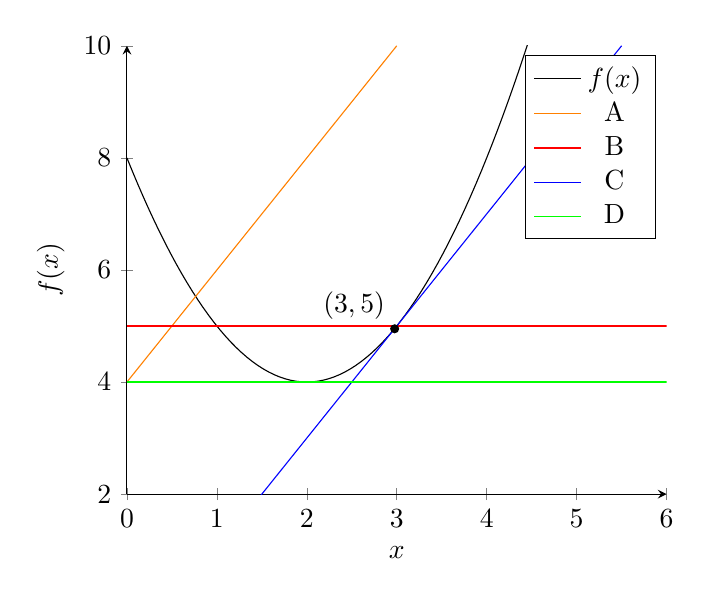
\begin{tikzpicture}
\begin{axis}[
    axis lines = left,
    xlabel = $x$,
    ylabel = {$f(x)$},
    xmin=0, xmax=6,
    ymin=2, ymax=10,
    ]
%Below the black parabola is defined
\addplot [
    domain=0:6, 
    samples=100, 
    color=black,
]
{x^2 - 4*x +8};
\addlegendentry{$f(x)$}

%Below the A approximation is defined
\addplot [
    domain=0:3, 
    samples=100, 
    color=orange,
]
{2*x +4};
\addlegendentry{A}

%Below the B approximation is defined
\addplot [
    domain=0:6, 
    samples=100, 
    color=red,
]
{0*x +5};
\addlegendentry{B}

%Below the C approximation is defined
\addplot [
    domain=-1.5:5.5, 
    samples=100, 
    color=blue,
]
{2*x -1};
\addlegendentry{C}

%Below the D approximation is defined
\addplot [
    domain=0:6, 
    samples=100, 
    color=green,
]
{0*x +4};
\addlegendentry{D}
\end{axis}

% points
\foreach \Point/\PointLabel in {(3.40,2.1)/{(3,5)}}
\draw[fill=black] \Point circle (0.05) node[above left] {$\PointLabel$};
\end{tikzpicture}


As approximations of the curve $f(x)$ at $x=3$,\\
\begin{itemize}
\item the error of Line A (given by $y=2x+4$, in orange) is $\answer{5}$\\
\item the error of Line B (given by $y=5$, in red) is $\answer{0}$\\
\item the error of Line C (given by $y=2x-1$, in blue) is $\answer{0}$\\
\item the error of Line D (given by $y=4$, in green) is $\answer{1}$\\
\end{itemize}

\begin{hint}
The error from an approximation is the distance between the true solution and the approximation
\end{hint}
\begin{hint}
If you are approximating $f(x)$ at $x=3$, then the `true solution' is the true value of $f(x)$ at $x=3$, AKA $f(3)$.
\end{hint}
\begin{hint}
The approximation of function $f(x)$ at $x=a$ using a line $y=mx+b$ is $ma+b$.
\end{hint}
\begin{hint}
Error shouldn't be negative. If you are finding the difference
between two numbers and the difference is negative, then the absolute
value of the difference would give the distance between the points.
\end{hint}
\end{question}

\begin{question}
Given the errors you found for $f(x)$ at $x=3$ using  each line (A,B,C, and D), which line(s) has the least error at $x=3$?
\begin{selectAll}
\choice{A}
\choice[correct]{B}
\choice[correct]{C}
\choice{D}
\end{selectAll}
\end{question}

This establishes an important property of a linear approximation
of a function at a given point: {\it the best linear approximation
should agree with the point at which you are approximating.}
In other words, if you are approximating a function $f(x)$ with a
line $\l(x)$ at $x=a$, then the line should be such that $\l(a)=f(a)$:
the output of the line is the same as the function's output at the $x$-value you are approximating from.\\

%%% Justifying the slope of the approximation
\underline{Question}: What is the difference between two lines that both
have no error where you are approximating at?
Consider the graph of $f(x)= (x-2)^2 + 4$ (in black), and three other linear approximations.

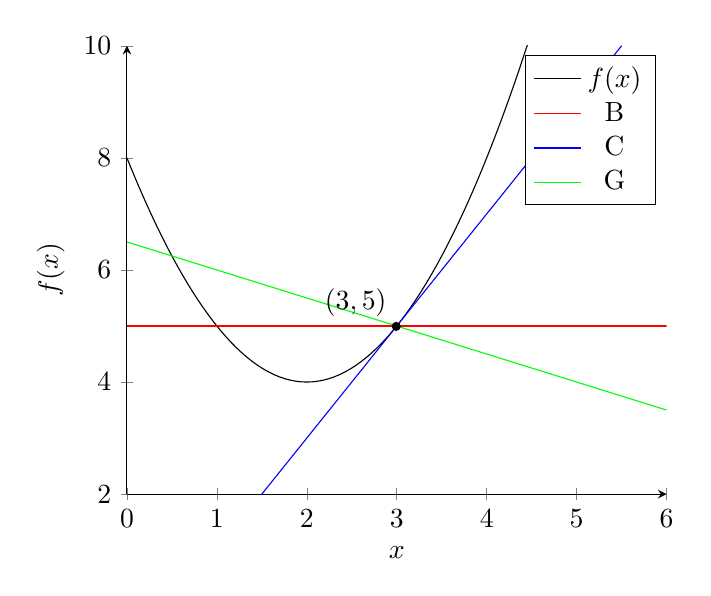
\begin{tikzpicture}
\begin{axis}[
    axis lines = left,
    xlabel = $x$,
    ylabel = {$f(x)$},
    xmin=0, xmax=6,
    ymin=2, ymax=10,
    ]
%Below the black parabola is defined
\addplot [
    domain=0:6, 
    samples=100, 
    color=black,
]
{x^2 - 4*x +8};
\addlegendentry{$f(x)$}

%Below the B approximation is defined
\addplot [
    domain=0:6, 
    samples=100, 
    color=red,
]
{0*x +5};
\addlegendentry{B}

%Below the C approximation is defined
\addplot [
    domain=-1.5:5.5, 
    samples=100, 
    color=blue,
]
{2*x -1};
\addlegendentry{C}

%Below the G approximation is defined
\addplot [
    domain=0:6, 
    samples=100, 
    color=green,
]
{-0.5*x +6.5};
\addlegendentry{G}
\end{axis}

% points
\foreach \Point/\PointLabel in {(3.42,2.13)/{(3,5)}}
\draw[fill=black] \Point circle (0.05) node[above left] {$\PointLabel$};
\end{tikzpicture}

Let's ask another question: What are the errors of the approximations `near' $x=3$? \\

As approximations of the curve $f(x)$ at {\bf $x=2.9$}, (Note that the )
\begin{itemize}
\item the error of Line B (given by $y=5$, in red) is $\answer{0.19}$
\item the error of Line C (given by $y=2x-1$, in blue) is $\answer{0.01}$
\item the error of Line G (given by $y=-0.5*x + 6.5$, in green) is $\answer{0.24}$
\end{itemize}

\[
\graph{f(x) = (x-2)^2 + 4, B(x) = 0*x + 5, C(x) = 2*x -1, G(x) = -0.5*x + 6.5, E = |f(2.9) - B(2.9)|}
\]

As approximations of the curve $f(x)$ at {\bf $x=3.1$},\\
\begin{itemize}
\item the error of Line B (given by $y=5$, in red) is $\answer{0.21}$\\
\item the error of Line C (given by $y=2x-1$, in blue) is $\answer{0.01}$\\
\item the error of Line G (given by $y=-0.5*x + 6.5$, in green) is $\answer{0.26}$\\
\end{itemize}
\[
\graph{f(x) = (x-2)^2 + 4}
\]




%%%% Towards defining a general rule for linear approximations

Given a line with slope $m$ through the point $(a, b)$, what is the point-slope form of the line?
\[
y = \answer[given]{m(x - a) + b}
\]

What is the slope of the line tangent to $f(x)$ at $x=3$?
\[
\answer{2}
\]

\begin{problem}
What point should an approximation of $f(x)$ at $x=3$ go through?

\[
(\answer[given]{3}, \answer[given]{5})
\]
\begin{hint}
Should the linear approximation go through the point at which it is approximating?
\end{hint}
\begin{hint}
Remember a point is an $(x,y)$ pair.
\end{hint}
\end{problem}

\begin{problem}
What is the equation of the line tangent to $f(x)$ at $x=3$?
\[
y = \answer[given]{2}x + \answer[given]{-1}
\]
\begin{hint}
Think $y=mx+b$
\end{hint}
\begin{hint}
What should the slope of the line be? (what is $m$?)
\end{hint}
\begin{hint}
It may be helpful to use point slope form first ($y=m(x-a) + b$) first,
and then convert into slope intercept form ($y=mx+b$).
\end{hint}

\begin{feedback}
Your line should look like this.
\[
\graph{f(x) = (x-2)^2+4, y = 2(x-3) + 5}
\]
\end{feedback}
\end{problem}




%\section{Linear approximation}
Given a function, a \textit{linear approximation} (at $x=x_0$) is a fancy phrase
for something you already know:
\begin{center}
\begin{quote}
  \textbf{The line tangent to the function (at $x=x_0$).}
\end{quote}
\end{center}


\begin{definition}\index{linear approximation}
If $f$ is a differentiable function at $x=a$, then a \textbf{linear
  approximation} for $f$ at $x=a$ is given by
\[
\l(x) = f'(a)(x-a) +f(a).
\]
\end{definition}


Note that $\l(x)$ is just the line tangent to $f(x)$ at $x=a$.


\begin{example}
Below is the graph of $f(x) = 1/8x^3 + (3/8)x^2 -3/4 - 2$ and the line
tangent to $f(x)$ at $x=a$. Feel free to explore how the tangent line
(in purple) changes as $a$ varies by using the slider. You may need to
hit `-' (zoom out) in order to see the linear approximations for large $a$ values.
\[
\graph[panel]{a=1, f(x) = 1/8x^3 + (3/8)x^2 -3/4 - 2, t(x) = f'(a)(x-a)+ f(a)}
\]

Notice how the linear approximation (the purple line) hugs
$f(x)$ (the green line) at the $x=a$ value!
\end{example}

A linear approximation of $f$ is a ``good'' approximation as long as
$x$ is ``not too far'' from $a$.
If one ``zooms in'' on $f$ at $x=a$ sufficiently, then $f$ and the linear
approximation are nearly indistinguishable. As a first example, we
will see how linear approximations allow us to make approximate
``difficult'' computations.




%%%%%% Aproximation of \sqrt[3]{50} number 1
\begin{example}
Use a linear approximation of $f(x) =\sqrt[3]{x}$ at $x=64$ to
approximate $\sqrt[3]{50}$.
\begin{explanation}
To start, write
\[
\ddx f(x) = \ddx x^{1/3} = \frac{1}{\answer[given]{3x^{2/3}}}.
\]
So our linear approximation is
\begin{align*}
\l(x) &= \frac{1}{3\cdot 64^{2/3}} (x-64) + \answer[given]{4} \\
&= \frac{1}{\answer[given]{48}} (x-64) + 4\\
&= \answer[given]{1/48}x + \answer[given]{8/3}.
\end{align*}




\[
\graph[panel]{}
\]


\textbf{Question. } Using the linear approximation just found (and the Desmos calculator above), 

\[
\sqrt[3]{50} \approx \answer[tolerance=0.000001]{3.70833333}.
\]
\begin{expandable}
Hint: Remember to round to 6 decimal places.
\end{expandable}



\begin{image}
\begin{tikzpicture}
	\begin{axis}[
            xmin=1,xmax=100,ymin=0,ymax=5,
            axis lines=center,
            xlabel=$x$, ylabel=$y$,
            every axis y label/.style={at=(current axis.above origin),anchor=south},
            every axis x label/.style={at=(current axis.right of origin),anchor=west},
          ]        
          \addplot [very thick, penColor, samples=150,smooth,domain=(0:100)] {x^(1/3))};
          \addplot [very thick, penColor2, domain=(0:100)] {x/48+8/3};
          \addplot [textColor,dashed] plot coordinates {(64,0) (64,4)};
          \addplot [textColor,dashed] plot coordinates {(0,4) (64,4)};
          \node at (axis cs:20,2.3) [penColor] {$f$};
          \node at (axis cs:20,3.3) [penColor2] {$\l$};
          \addplot[color=penColor3,fill=penColor3,only marks,mark=*] coordinates{(64,4)};  %% closed hole            
        \end{axis}
\end{tikzpicture}
\end{image}

Now let's use our approximation and true value to find our approximation's error.


Use the Desmos widget below to determine the error of your approximation for $\sqrt[3]{50}$, noting that $\sqrt[3]{50} = f(50)$.

\[
\graph[panel]{f(x) = x^{1/3}, l(x) = (1/48) x + (8/3)}
\]

\textbf{Question. } The approximation is \wordChoice{\choice[correct]{above}\choice{below}} the true 
answer by $\answer[tolerance=0.000001]{0.024302}$ units.

\begin{expandable}
Hint: Note that $f(50)$ when plugged into Desmos will give $sqrt[3]{50}$.
\begin{expandable}
What will be $\l(50)$ give you in the Desmos calculator?
\begin{expandable}
How can you use the Desmos calculator to find the difference of these two numbers?
\begin{expandable}
What does $f(50)-\l(50)$ give you? Is that what you want?
\end{expandable}
\end{expandable}
\end{expandable}
\end{expandable}

\end{explanation}
\end{example}

With modern calculators and computing software it may not appear
necessary to use linear approximations. In fact they are quite
useful. In cases requiring an explicit numerical approximation, they
allow us to get a quick rough estimate which can be used as a
``reality check'' on a more complex calculation. In some complex
calculations involving functions, the linear approximation makes an
otherwise intractable calculation possible, without serious loss of
accuracy.



%% Approximation using cube root of 27 instead.
\begin{example}
Now use a linear approximation of $f(x) =\sqrt[3]{x}$ at $\underline{x=27}$ to
approximate $\sqrt[3]{50}$.
\begin{explanation}
To start, write
\[
\ddx f(x) = \ddx x^{1/3} = \frac{1}{\answer[given]{3x^{2/3}}}.
\]
By using our formula for linear approximations, our linear 
approximation for $f(x)=\sqrt[3]{x}$ at $x=27$ is
\begin{align*}
m(x) &= \answer[given]{1/27}x + \answer[given]{2}.
\end{align*}


\textbf{Question. } Using the linear approximation just found (and the Desmos calculator below),
\[
\sqrt[3]{50} \approx \answer[tolerance=0.0000005]{3.851852}.
\]
\begin{expandable}
Remember to round to 6 decimal places.
\end{expandable}

\[
\graph[panel]{}
\]




\begin{image}
\begin{tikzpicture}
	\begin{axis}[
            xmin=1,xmax=100,ymin=0,ymax=5,
            axis lines=center,
            xlabel=$x$, ylabel=$y$,
            every axis y label/.style={at=(current axis.above origin),anchor=south},
            every axis x label/.style={at=(current axis.right of origin),anchor=west},
          ]        
          \addplot [very thick, penColor, samples=150,smooth,domain=(0:100)] {x^(1/3))};
          \addplot [very thick, penColor2, domain=(0:100)] {x/27+2};
          \addplot [textColor,dashed] plot coordinates {(27,0) (27,3)};
          \addplot [textColor,dashed] plot coordinates {(0,3) (27,3)};
          \node at (axis cs:50,3.3) [penColor] {$f$};
          \node at (axis cs:50,4.3) [penColor2] {$m$};
          \addplot[color=penColor3,fill=penColor3,only marks,mark=*] coordinates{(27,3)};  %% closed hole            
        \end{axis}
\end{tikzpicture}
\end{image}

Now let's use our approximation and true value to find our approximation's error.

Use the Desmos widget below to determine the error of your approximation for $\sqrt[3]{50}$, noting that $\sqrt[3]{50} = f(50)$.

\[
\graph[panel]{f(x) = x^{1/3}, m(x) = (1/27) x + 2}
\]


\textbf{Question. } The approximation is \wordChoice{\choice[correct]{above}\choice{below}} the true 
answer by $\answer[tolerance=0.000001]{0.167820}$ units.

\begin{expandable}
Hint: Note that $f(50)$ when plugged into Desmos will give $sqrt[3]{50}$.
\begin{expandable}
What will be $m(50)$ give you in the Desmos calculator?
\begin{expandable}
How can you use the Desmos calculator to find the difference of these two numbers?
\begin{expandable}
What does $f(50)-m(50)$ give you? Is that what you want?
\end{expandable}
\end{expandable}
\end{expandable}
\end{expandable}

\end{explanation}
\end{example}

Notice that we approximated $\sqrt[3]{50}$ using two different
linear approximations of $\sqrt[3]{x}$ and hence got two different
approximations of $\sqrt[3]{50}$.

%%% Comparison of approximations
\begin{question}
Compare your linear approximations when using $x=64$ and $x=27$. Which linear approximation of $\sqrt[3]{x}$ gives a better approximation of $\sqrt[3]{50}$?

\begin{multipleChoice}
   \choice{The approximation using $x=27$, because $27$ is closer to $50$ than $64$.}
   \choice{The approximation using $x=27$, because $64$ is closer to $50$ than $27$.}
   \choice[correct]{The approximation using $x=64$, because $64$ is closer to $50$ than $27$.}
   \choice{The approximation using $x=64$, because $27$ is closer to $50$ than $64$.}
\end{multipleChoice}

\begin{image}
\begin{tikzpicture}
	\begin{axis}[
            xmin=20,xmax=70,ymin=2.5,ymax=4.5,
            axis lines=center,
            xlabel=$x$, ylabel=$y$,
            every axis y label/.style={at=(current axis.above origin),anchor=south},
            every axis x label/.style={at=(current axis.right of origin),anchor=west},
          ]        
          \addplot [very thick, penColor, samples=250,smooth,domain=(20:70)] {x^(1/3))};
          \addplot [very thick, penColor2, domain=(20:70)] {x/27+2};
          \addplot [very thick, penColor4, domain=(20:70)] {x/48+8/3};
          \addplot [textColor,dashed] plot coordinates {(50,0) (50,3.68403149864)};         
          \node at (axis cs:42,3.1) [penColor] {$f$};
          \node at (axis cs:55,4.2) [penColor2] {$m$};
          \node at (axis cs:35,3.5) [penColor4] {$\l$};
          \addplot[color=penColor3,fill=penColor3,only marks,mark=*] coordinates{(50,3.68403149864)};  %% closed hole            
        \end{axis}
\end{tikzpicture}
\end{image}

As a warning: not all approximations are over estimates! This just came about
from this example. Some linear approximations are over-estimates. Some are
under-estimates. Some vary for different points you are approximating at!
\end{question}





%% Approximation for sine function
\begin{example}
Use a linear approximation of $f(x) =\sin(x)$ at $x=0$ to approximate
$\sin(0.3)$.
\begin{explanation}
To start, write
\[
\ddx f(x) = \answer[given]{\cos(x)},
\]
so our linear approximation is
\begin{align*}
\l(x) &= \answer[given]{\cos(0)}\cdot(x-\answer[given]{0}) + \answer[given]{0}\\
&= \answer[given]{x}.
\end{align*}
\begin{image}
%\begin{marginfigure}
\begin{tikzpicture}
	\begin{axis}[
            xmin=-1.6,xmax=1.6,ymin=-1.5,ymax=1.5,
            axis lines=center,
            xtick={-1.57, 0, 1.57},
            xticklabels={$-\pi/2$, $0$, $\pi/2$},
            ytick={-1,1},
            unit vector ratio*=1 1 1,
            xlabel=$x$, ylabel=$y$,
            every axis y label/.style={at=(current axis.above origin),anchor=south},
            every axis x label/.style={at=(current axis.right of origin),anchor=west},
          ]        
          \addplot [very thick, penColor, samples=100,smooth, domain=(-1.6:1.6)] {sin(deg(x))};
          \addplot [very thick, penColor2, samples=100,smooth] {x};
          \node at (axis cs:1,.6) [penColor] {$f$};
          \node at (axis cs:-1,-1.2) [penColor2] {$\l$};
          \addplot[color=penColor3,fill=penColor3,only marks,mark=*] coordinates{(0,0)};  %% closed hole          
        \end{axis}
\end{tikzpicture}
%\caption{A linear approximation of $f(x) = \sin(x)$ at $x=0$.}
%\label{figure:la sin}
%\end{marginfigure}
\end{image}
Hence the linear approximation for $\sin(x)$ at $x=0$ is $\l(x) = x$,
and so $\l(0.3) = 0.3$.  Comparing this to $\sin(.3) \approx 0.295$,
we see that the approximation is quite good. For this reason, it is common
to approximate $\sin(x)$ with its linear approximation $\l(x) = x$
when $x$ is near zero.  
%see Figure~\ref{figure:la sin}.
\end{explanation}
\end{example}





\end{document}